% 8185: Quant Bhandari PS1

\documentclass[12pt]{article}
%\usepackage[T1]{fontenc}
%\usepackage{lipsum}
\renewcommand{\baselinestretch}{1.2} 
\usepackage{graphicx}
\usepackage{hyperref}
\hypersetup{
    colorlinks=true,
    urlcolor=blue,
    citecolor=blue
}
\usepackage[export]{adjustbox}
\usepackage{subcaption}
\usepackage{amsmath}
\usepackage{amssymb}
\usepackage{amsfonts}
\usepackage{geometry}
\setcounter{MaxMatrixCols}{20}
\geometry{a4paper,
 left=3cm,right=3cm,
 top=1.5cm, bottom=1.5cm}

\usepackage{natbib}
\bibliographystyle{apalike}

%\usepackage{natbib}
%setcitestyle{authoryear,open={(},close={)}}
\graphicspath{ {../figs/} }

\begin{document}
%\thispagestyle{myheadings}
%\markright{Indian Statistical Institute, New Delhi\hfill }

\title{Econ 8185 (002): Quant PS1}
\author{Bipul Verma}
\date{\today}
\maketitle

%\tableofcontents{}
\abstract{This document applies Kalman Filter, EM algorithm to US gdp data.}

\vspace{8cm}

%\begin{center}
%\includegraphics[scale=0.4]{isi_logo.png}
%\end{center}
%\begin{center}
%\begin{Large}
%INDIAN STATISTICAL INSTITUTE, NEW-DELHI.
%\end{Large}
%\end{center}


\newpage

\section{US GDP growth rate}
The GDP growth rate is given by the following formula:
\begin{align*}
g_t = \frac{Y_{t+1} - Y_{t}}{Y_t}
\end{align*}
Another equivalent way to calculate the growth rate is to take differences of logs. This follows since:
\begin{align*}
log(Y_{t+1}) - log(Y_t) & = log(\frac{Y_{t+1}}{Y_t})\\
& = log(1 + \frac{Y_{t+1}}{Y_t} -1) \\
& = log(1 + g_t) \\
& \approx g_t.
\end{align*}

\begin{figure}[h]
\centering
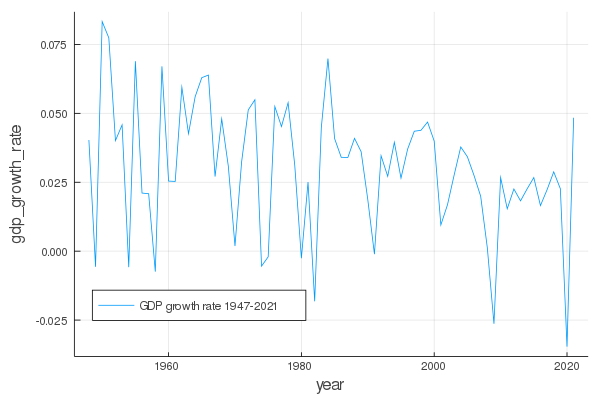
\includegraphics[scale=0.5]{gdp_growth.png}
\caption{US GDP growth rate 1947-2021}
\end{figure}

\section*{Summary of Kalman Filter, Smoother, and EM Algorithm}
Consider the following state space system:
\begin{gather*}
x_{t} = B x_{t-1} + w_{t}\\
y_t = Z x_t + v_t \\
w_t \sim N(0, Q) \\
v_t \sim N(0, R).
\end{gather*} 

\subsection{Kalman Filter}
Kalman filter gives the prediction of state and its update based on past value of observable. \\
\textbf{Notations:}
\begin{align*}
& \hat{x}_{t-1|t-1} = \mathbb{E}[x_{t-1}|y^{t-1}]\\
& P_{t-1|t-1} = \mathbb{E}[(x_{t-1}-\hat{x}_{t-1|t-1})(x_{t-1} - \hat{x}_{t-1|t-1})' |y^{t-1}]\\
& \hat{x}_{t|t-1} = \mathbb{E}[x_{t}|y^{t-1}]\\
& P_{t|t-1} = \mathbb{E}[(x_{t}-\hat{x}_{t|t-1})(x_{t} - \hat{x}_{t|t-1})' |y^{t-1}]
\end{align*}
\textbf{Initialization:}
Set $\hat{x}_{1|0} = x_0$ and $P_{1|0} = P_0$.\\
\textbf{Filtering Algorithm (Forward Pass) $t \geq 1$:}
\begin{align*}
& \kappa_t = P_{t|t-1}Z'(ZP_{t|t-1}Z' + R)^{-1}\\
& \hat{x}_{t|t} = \hat{x}_{t|t-1} + \kappa_t(y_t - Z\hat{x}_{t|t-1})\\
& P_{t|t} = P_{t|t-1} - \kappa_tZP_{t|t-1} \\
& \hat{x}_{t+1|t} = B \hat{x}_{t|t} \\
& P_{t+1|t} = BP_{t|t}B' + Q 
\end{align*}

\subsection{Kalman Smoother:}
The estimates of states from the Kalman Filter will feed into the Kalman Smoother to obtain estimates based on all values of observable.\\
\textbf{Notations:}
\begin{align*}
& \hat{x}_{t|T} = \mathbb{E}[x_{t}|Y]
\end{align*}
\textbf{Smoothing Algorithm (Backward Pass):}
\begin{align*}
& J_t = P_{t|t}B'P_{t+1|t}^{-1} \\
& \hat{x}_{t|T} = \hat{x}_{t|t} + J_t(\hat{x}_{t+1|T} - \hat{x}_{t+1|t})\\
& P_{t|T} = P_{t|t} + J_t(P_{t+1|T} - P_{t+1|t})J_t' \\
& P_{t, t-1|T} = J_{t-1}P_{t|T}
\end{align*}

\subsection{EM Algorithm}
For the purpose of current exercise we'll write down the update equation for $Q$ and $R$ only. Note that the expectations are conditional on $(Y, \theta_j)$.\\
\textbf{Parameter Update Equation:}
\begin{align*}
& Q_{j+1} = \frac{1}{T-1} \sum_{t=2}^{T}(\mathbb{E}[x_tx_t'] - \mathbb{E}[x_t x_{t-1}']B' - B\mathbb{E}[x_{t-1} x_t' ] + B\mathbb{E}[x_{t-1}x_{t-1}']B')\\
& R_{j+1} = \frac{1}{T} \sum_{t=1}^{T}(\mathbb{E}[y_t y_t'] - \mathbb{E}[y_tx_t']Z' - Z\mathbb{E}[x_ty_t'] + Z \mathbb{E}[x_tx_t']Z') \\
\end{align*}
 The update equations are sometimes written in the following form as well:
\begin{align*}
& Q_{j+1} = \frac{1}{T-1} \Bigg( \sum_{t=2}^{T} \mathbb{E}[x_tx_t'] - \Big(\sum_{t=2}^{T} \mathbb{E}[x_tx_{t-1}']\Big) \Big(\sum_{t=2}^{T} \mathbb{E}[x_{t-1}x_{t-1}']\Big)^{-1}\Big(\sum_{t=2}^{T} \mathbb{E}[x_{t-1}x_t']\Big) \Bigg)\\
& R_{j+1} =\frac{1}{T}\Bigg( \sum_{t=1}^{T} \mathbb{E}[y_ty_t'] - \Big( \sum_{t=1}^{T} \mathbb{E}[y_tx_{t}']\Big)\Big(\sum_{t=1}^{T} \mathbb{E}[x_{t}x_{t}']\Big)^{-1}\Big(\sum_{t=1}^{T} \mathbb{E}[x_{t}y_t']\Big) \Bigg).
\end{align*}
The conditional expectations in the update equation can be evaluated from the Kalman Smoother output as follows:
\begin{align*}
& \mathbb{E}[x_tx_t'|Y, \theta_j] = P_{t|T} + \hat{x}_{t|T}\hat{x}_{t|T}' \\
& \mathbb{E}[x_tx_{t-1}'| Y, \theta_j] = P_{t, t-1|T} + \hat{x}_{t|T}\hat{x}_{t-1|T}'
\end{align*}

\subsubsection{Implementation of EM Algorithm}
To understand the implementation we introduce some additional notations for clarity. \\
\textbf{Notations:}
\begin{align*}
& \alpha_t =\mathbb{E}[y_ty_t'|Y, \theta_j] \\
& \delta_t = \mathbb{E}[y_tx_t'|Y, \theta_j] \\
& \gamma_t = \mathbb{E}[x_tx_t'|Y, \theta_j] \\
& \beta_t = \mathbb{E}[x_tx_{t-1}'|Y, \theta_j].
\end{align*}
All the above mentioned expectations can be calculated from the output of Kalman Smoother as outlined in the previous section. The update equations using the above notation is given below.\\
\textbf{Update Equation:}
\begin{align*}
& Q_{j+1} = \frac{1}{T-1} \sum_{t=2}^{T}(\gamma_t - \beta_tB' - B\beta_t' + B\gamma_{t-1}B')\\
& R_{j+1} = \frac{1}{T} \sum_{t=1}^{T}(\alpha_t - \delta_tZ' - Z\delta_t' + Z \gamma_tZ') 
\end{align*}
The update equations are sometimes written in the following form as well. Writing the update equation in the below form requires making use of some trace manipulations.
\begin{align*}
& Q_{j+1} = \frac{1}{T-1} \Bigg( \sum_{t=2}^{T} \gamma_t - \Big(\sum_{t=2}^{T}\beta_t \Big) \Big(\sum_{t=2}^{T} \gamma_{t-1}\Big)^{-1}\Big(\sum_{t=2}^{T}\beta_t\Big)' \Bigg)\\
& R_{j+1} =\frac{1}{T}\Bigg( \sum_{t=1}^{T} \alpha_t - \Big( \sum_{t=1}^{T} \delta_t \Big)\Big(\sum_{t=1}^{T} \gamma_t \Big)^{-1}\Big(\sum_{t=1}^{T} \delta_t\Big) \Bigg).
\end{align*}


\section{Applying Kalman Filter to change in log output}
Define: $$y_t =log(Y_{t+1}) - log(Y_t).$$ It is given that $y_t$ follows the following process:
\begin{align}
y_t = Z \mu_t + \sigma_{\epsilon}\epsilon_t\\
\mu_{t+1} = B \mu_t + \sigma_{\nu}\nu_{t+1}
\end{align}
For the present case $B=[1], Z = [1], Q = \sigma_{\nu}^2, R = \sigma_{\epsilon}^2$.

\subsection{Simulated State}
In the gaussian case the best guess for $\mu_t$ given $y^{t-1}$ is given by $\mathbb{E}[\mu_t| y^{t-1}]$. For the present case we set the values $\sigma_{\nu} = 0.15, \sigma_{\epsilon} = 0.10$. We plot the values for  $\mathbb{E}[\mu_t| y^{t-1}]$ below:
\begin{figure}[h]
\centering
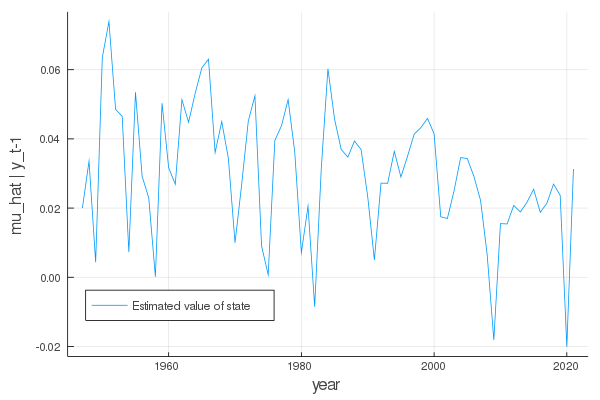
\includegraphics[scale=0.5]{2_a.png}
\caption{Estimated Value of State}
\end{figure}


\subsection{Test Case}
For this case we simulate the values for $\mu_t, y_t$ using the parameter values same as in the previous part. We then calculate $\mathbb{E}[\mu_t|y^{t-1}]$ and compare it with the actual values. The following figure graphs the estimates:
\begin{figure}[h]
\centering
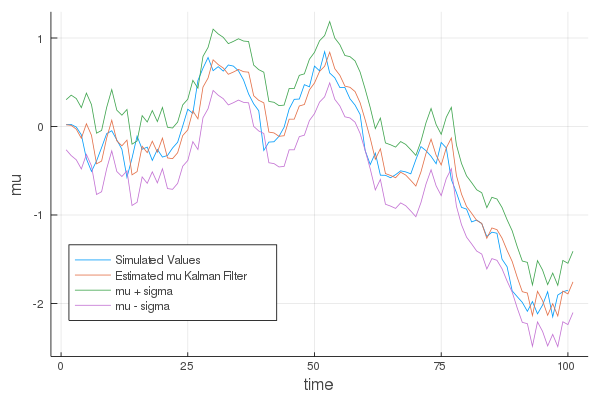
\includegraphics[scale=0.5]{2_b.png}
\caption{Estimated vs Simulated Values}
\end{figure}

\newpage

\section{MLE estimation}
We use the following formula for MLE estimation of $sigma_{\nu}, \sigma_{\epsilon}$ based on the actual data for $y_t$:
\begin{align*}
\ln L = \sum_t \{ -\frac{n}{2} \ln 2\pi -\frac{1}{2}\ln |det(F_t)| - \frac{1}{2}i_t'F_t^{-1}i_t 
\end{align*}

The estimates are: $\hat{\sigma}_{\nu} = 0.00161 , \hat{\sigma}_{\epsilon} =  0.0224$. Using these estimates we now graph $\mathbb{E}[\hat{\mu}_{t+1}|y^{t-1}]$.
\begin{figure}[h]
\centering
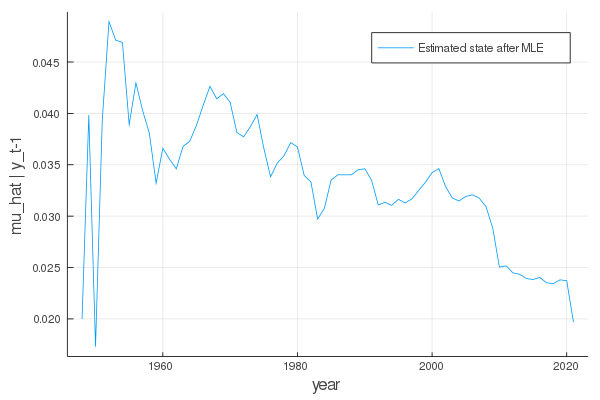
\includegraphics[scale=0.5]{3_b.png}
\caption{Estimated Value of State}
\end{figure}


\section{EM Method}
We follow Holmes E. E. (2012) to implement the EM algorithm.
For the present case $B = [1]$ and $Z = [1]$. The EM algorithm is an iterative algorithm, where the new set of parameters maximizes the Expected value of log likelihood. The estimates from EM are: $\hat{\sigma}_{\nu} = 0.0196, \hat{\sigma}_{\epsilon} = 0.0176$. \\

\textbf{Note:} \textit{We checked out EM algorithm for the simulated case. There both MLE estimates and EM estimates coincides. This leads us to conclude that our MLE and EM algorithm are being implemented correctly. However, the MLE and EM estimates are different when run on actual data. This may be because of low number of data points for actual growth rate data. It is also to note that the variance of growth rate is very small $(0.000547)$, which might lead to imprecise estimates.}



%%--------REFERENCES---------------%%
% https://users.ece.cmu.edu/~byronyu/papers/derive_ks.pdf
% https://web.stanford.edu/~lmackey/stats306b/doc/stats306b-spring14-lecture11_scribed.pdf
% https://jeti.uni-freiburg.de/papers/1-s2.0-S0096300314006869-main.pdf
% https://citeseerx.ist.psu.edu/viewdoc/download?doi=10.1.1.314.2260&rep=rep1&type=pdf

%\newpage
%\bibliography{ref}

\end{document}